\section{Exigences spécifiques}

L'utilisateurs peut interagir avec le robot dans le biais de l'utilisation d'un smartphone avec l'application télécommande développer sous Android. L'utilisateur pourra alors par le biais d'une interface graphique interagir avec le robot. 

\subsection{Interfaces homme-machine partie Android}

\subsubsection{Page principale}

\begin{figure}[H]
    \centering
    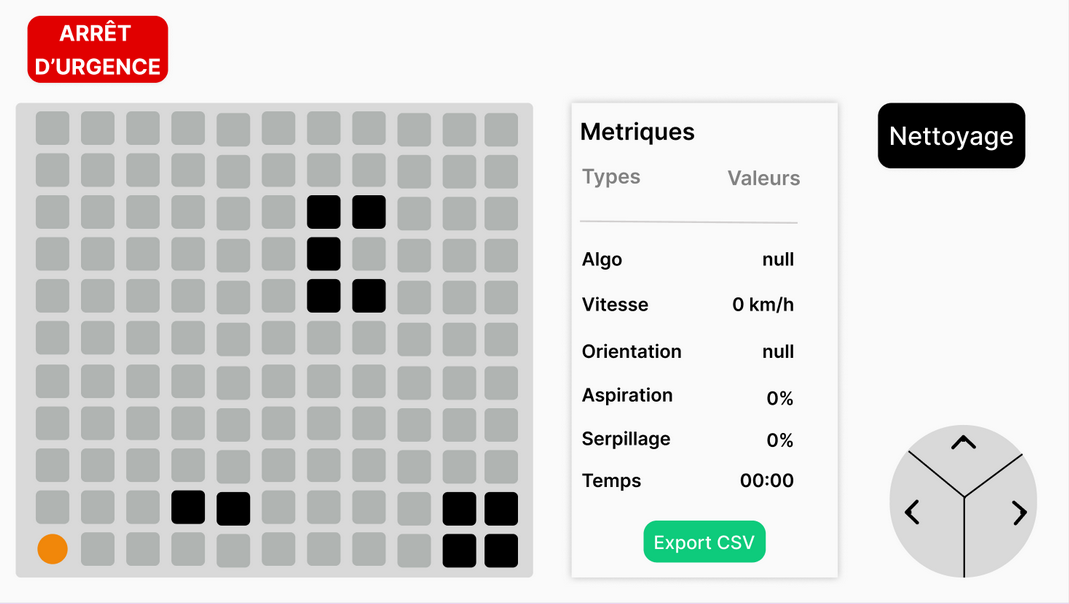
\includegraphics[scale=0.25]{data/IHM1.png}
    \caption{Page principale de l'application Android}
    \label{fig:ihm_android_main}
\end{figure}

Après l'étape de connexion on arrive sur la page principale de l'application. On y trouve un bouton d'arrêt d'urgence qui permettra d'arrêter tous les mouvements du robot, une carte qui représente le terrain dans lequel se déplace le robot des métriques sur le robot ainsi qu'un bouton nettoyage permettant de lancer la séquence de nettoyage automatique enfin un joystick qui permet d'avancer, tourner à droite ou à gauche. 

\subsubsection{Pop-up lancement Nettoyage}

\begin{figure}[H]
    \centering
    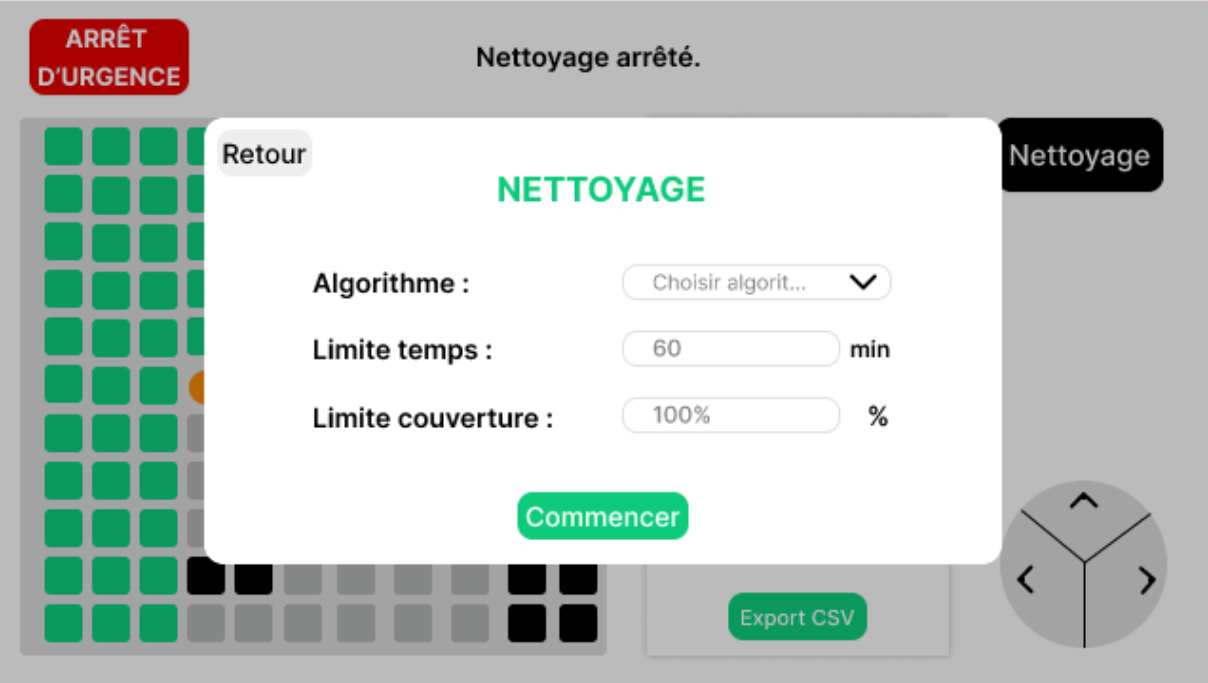
\includegraphics[scale=0.25]{data/IHM2.png}
    \caption{Pop-up de lancement du nettoyage}
    \label{fig:ihm_android_popup}
\end{figure}

Le pop-up du nettoyage apparaît quand on appui sur le bouton nettoyage, on y indique l'algorithme de nettoyage que l'on veut ainsi que la condition d'arrêt du nettoyage (sois une limite de temps ou/et un pourcentage de couverture de nettoyage).

\subsubsection{Arrêt d'urgence}

\begin{figure}[H]
    \centering
    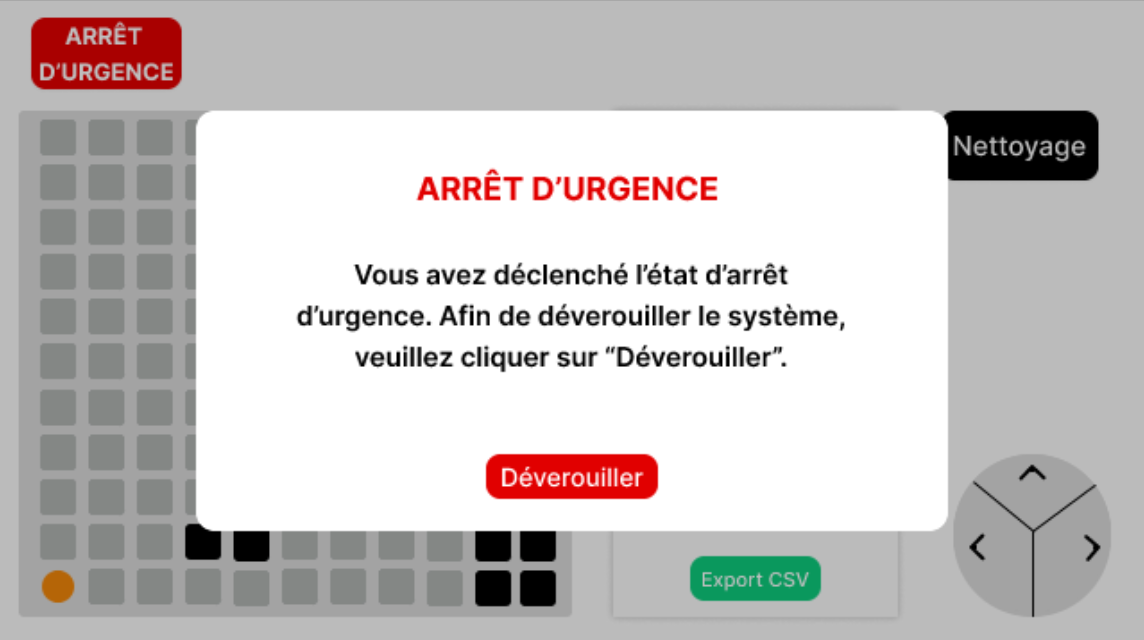
\includegraphics[scale=0.25]{data/IHM3.png}
    \caption{Pop-up d'arrêt d'urgence}
    \label{fig:ihm_android_emergency}
\end{figure}

Quand on appui sur le bouton arrêt d'urgence ce popup bloquant apparaît, les mouvements du robot sont bloqués et il faut appuyer sur le bouton déverrouiller pour revenir à l'état nominal. 

\subsubsection{Export CVS}

\begin{figure}[H]
    \centering
    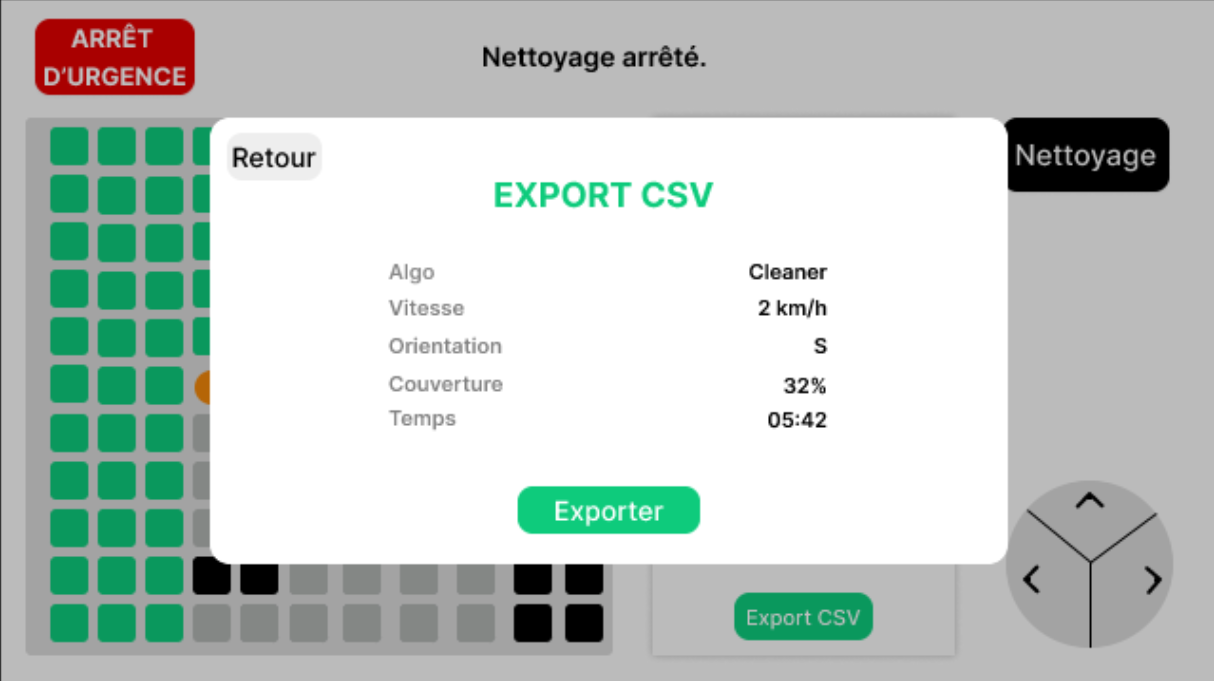
\includegraphics[scale=0.25]{data/IHM4.png}
    \caption{Pop-up d'export CVS}
    \label{fig:ihm_android_export}
\end{figure}

À tout moment, on créer un fichier avec tous les mouvements du robot l'algorithme utilisé plus des informations sur la batterie le temps d'exécution, la vitesse moyenne.

\subsubsection{Page de nettoyage}

\begin{figure}[H]
    \centering
    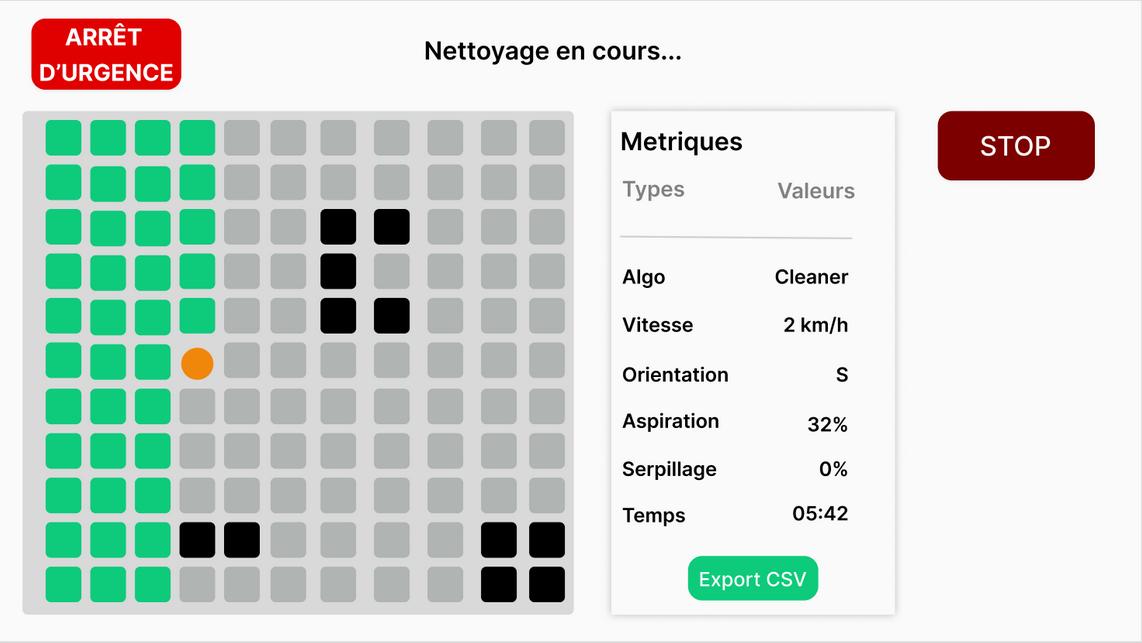
\includegraphics[scale=0.25]{data/IHM5.png}
    \caption{Page de nettoyage}
    \label{fig:ihm_android_cleaning}
\end{figure}

Sur cette page on retrouve l'arrêt d'urgence ainsi que la carte avec l'avancement en temps réel des mouvements des robots (aspiration, lavage), on peut appuyer sur le bouton stop pour arrêter le nettoyage et retourner en mode manuel. 

\subsection{Interfaces homme-machine partie C}

Après le lancement de l'application sur le robot cet écran s'affichera dans le terminal. 

\begin{figure}[H]
    \centering
    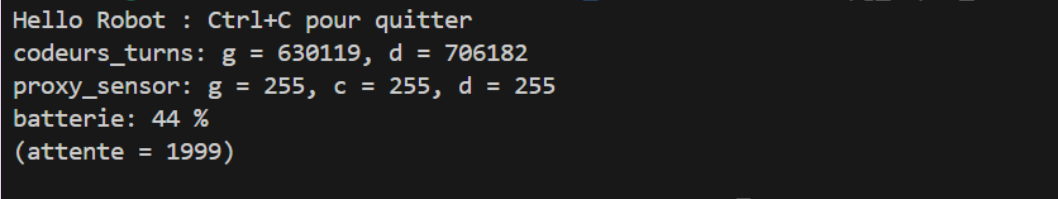
\includegraphics[scale=0.25]{data/IHM6.png}
    \caption{Interface C}
    \label{fig:ihm_c}
\end{figure}

On y retrouve le nombre de pas enregistré par les encodeurs, les états des capteurs de proximité et l'état de la batterie.

\subsection{Interfaces homme-machine partie Robot}

L'interface homme machine sur le robot correspond à une LED RVB. 

Les différents codes couleur cyclique sont décrit dans le tableau suivant : 

\begin{tabularx}{\textwidth}{|X|X|}
    \hline
    \textbf{Code Couleur} & \textbf{Signification} \\
    \hline
    MRPIZ\_E\_INIT (erreur d'initialisation)  & La LED clignote en rouge toute les une secondes  \\
    \hline
    MRPIZ\_E\_MOTOR\_CMD (commande moteur invalide)  & La LED clignote en bleu pendant 1 seconde puis en rouge pendant 1 seconde et est éteint 1 seconde  \\
    \hline
    MRPIZ\_E\_MOTOR\_ID (ID du moteur invalide)  & La LED clignote en vert pendant 1 seconde puis en rouge pendant 1 seconde et est éteint 1 seconde  \\
    \hline
    MRPIZ\_E\_PROXY\_SENSOR\_ID (Invalid Proxy sensor ID)  & La LED clignote en vert pendant 1 seconde puis en rouge pendant 1 seconde et est éteint 1 seconde  \\
    \hline
    MRPIZ\_E\_UART (erreur communication) & La LED clignote en rouge pendant 1 seconde, est éteint 1 seconde puis en vert à 3hz et est éteint 1 seconde \\
    \hline
    MRPIZ\_E\_SYSTEM (TBD) & TBD \\
    \hline
    ...\_E\_Remote\_CONNEXION\_FAILED & 1 seconde allumée en bleu puis 1 seconde éteinte \\
    \hline
    ...\_E\_Remote\_CONNEXION\_LOST & 1 seconde allumée à 3 Hz en bleu puis 1 seconde éteinte \\
    \hline
    ...\_E\_Remote\_EMERGENCY\_ENGAGED & 1 seconde allumée à 3 Hz en rouge puis 1 seconde allumée à 3 Hz en bleu puis 1 seconde éteinte \\
    \hline
\end{tabularx}

\subsection{Description des fonctions}

\subsubsection{Demande à passer en mode "Urgence"}

\begin{figure}[H]
    \centering
    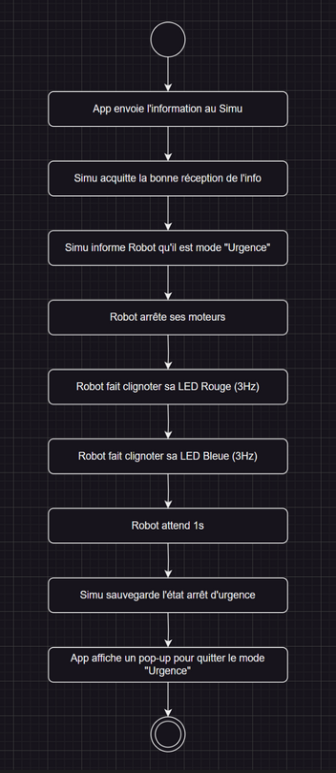
\includegraphics[scale=0.25]{data/function1.png}
    \caption{Fonction Demande de passage en mode "Urgence"}
    \label{fig:ihm_emergency}
    \end{figure}

\subsubsection{Demande un déplacement du robot}

\begin{figure}[H]
    \centering
    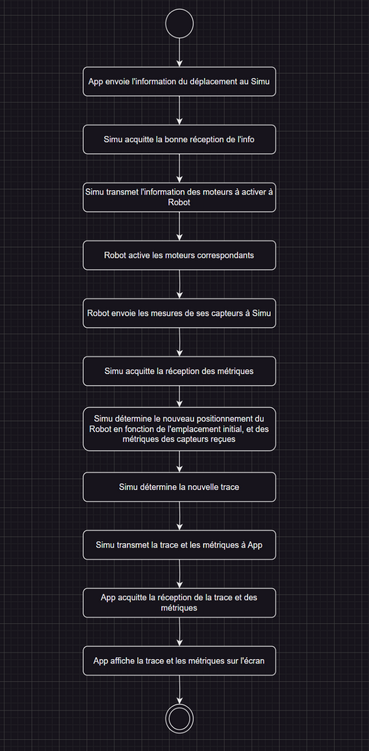
\includegraphics[scale=0.25]{data/function2.png}
    \caption{Fonction Demande de déplacement du robot}
    \label{fig:ihm_move}
\end{figure}

\subsubsection{Quitte App}

\begin{figure}[H]
    \centering
    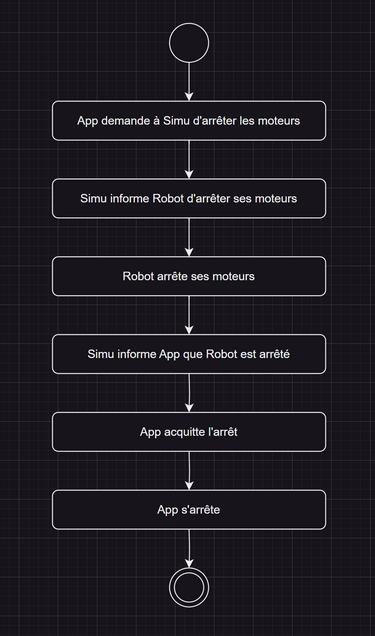
\includegraphics[scale=0.25]{data/function3.png}
    \caption{Fonction Quitte l'application}
    \label{fig:ihm_quit}
\end{figure}

\subsubsection{Récupère l'état du mode "Urgence"}

\begin{figure}[H]
    \centering
    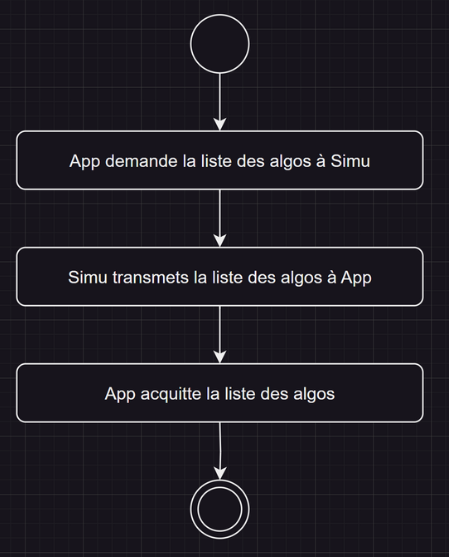
\includegraphics[scale=0.25]{data/function4.png}
    \caption{Fonction Récupère l'état du mode "Urgence"}
    \label{fig:ihm_get_emergency}
\end{figure}